% The Knowledge Pipeline — Atlas (COMBINED single-file build)
% All diagrams inlined as TikZ — no external PDFs required.
% Compile with: pdflatex atlas-combined.tex
\documentclass[11pt]{article}

\usepackage[a4paper, margin=1.6cm]{geometry}
\usepackage{graphicx}
\usepackage{adjustbox}
\usepackage{xcolor}
\usepackage{lmodern}
\usepackage[T1]{fontenc}
\usepackage[english]{babel}
\usepackage{amsmath}
\usepackage{amssymb}
\usepackage{tikz}
\usetikzlibrary{
    arrows.meta,
    backgrounds,
    calc,
    decorations.pathmorphing,
    decorations.pathreplacing,
    fadings,
    fit,
    positioning,
    shapes.geometric,
    shapes.symbols
}

%% ---------- Atlas colours ----------
\definecolor{ink}   {HTML}{1F2433}
\definecolor{accent}{HTML}{3A6E5B}
\definecolor{soft}  {HTML}{6B7280}
\definecolor{soft2} {HTML}{B0B6BF}

%% ---------- Diagram colours (merged from all sub-files) ----------
\definecolor{think}    {HTML}{4A6FA5}
\definecolor{thinkbg}  {HTML}{E8EEF7}
\definecolor{lens}     {HTML}{C8553D}
\definecolor{lensbg}   {HTML}{FBEBE6}
\definecolor{coil}     {HTML}{6B7280}
\definecolor{node}     {HTML}{2E3A59}
\definecolor{nodebg}   {HTML}{F2F4F8}
\definecolor{c1}{HTML}{4A6FA5}
\definecolor{c1bg}{HTML}{EBF1F9}
\definecolor{c2}{HTML}{C9883A}
\definecolor{c2bg}{HTML}{FBF2DD}
\definecolor{c3}{HTML}{B85C92}
\definecolor{c3bg}{HTML}{F8E8F0}
\definecolor{c4}{HTML}{4F8A6B}
\definecolor{c4bg}{HTML}{E7F0EA}
\definecolor{c5}{HTML}{C8553D}
\definecolor{c5bg}{HTML}{FBEBE6}
\definecolor{c6}{HTML}{5B6E8C}
\definecolor{c6bg}{HTML}{ECEFF4}
\definecolor{stagebg}    {HTML}{FBFCFE}
\definecolor{stageborder}{HTML}{C8CFDB}
\definecolor{accentbg}   {HTML}{E4EFE9}
\definecolor{kgbg}       {HTML}{FBFCFE}
\definecolor{kgborder}   {HTML}{C8CFDB}
\definecolor{ph1}{HTML}{4A6FA5}
\definecolor{ph1bg}{HTML}{EBF1F9}
\definecolor{ph2}{HTML}{C9883A}
\definecolor{ph2bg}{HTML}{FBF2DD}
\definecolor{ph3}{HTML}{4F8A6B}
\definecolor{ph3bg}{HTML}{E7F0EA}
\definecolor{t1bg}   {HTML}{FBFCFE}
\definecolor{t2bg}   {HTML}{F8F6F2}
\definecolor{t3bg}   {HTML}{F4F7F5}
\definecolor{tborder}{HTML}{D5DAE3}
\definecolor{phase1}     {HTML}{4A6FA5}
\definecolor{phase1bg}   {HTML}{EBF1F9}
\definecolor{phase2}     {HTML}{C9883A}
\definecolor{phase2bg}   {HTML}{FBF2DD}
\definecolor{phase3}     {HTML}{4F8A6B}
\definecolor{phase3bg}   {HTML}{E7F0EA}
\definecolor{execborder} {HTML}{C8CFDB}
\definecolor{execbg}     {HTML}{FBFCFE}

\pagestyle{empty}
\setlength{\parindent}{0pt}
\renewcommand{\arraystretch}{1.3}

\newcommand{\stage}[3]{%
    {\Large\color{accent}\textbf{Stage #1\,/\,#2}}\\[2pt]
    {\color{soft}\itshape #3}\par\vspace{8pt}%
}

\begin{document}


%% ============================================================
%% Title page
%% ============================================================
\thispagestyle{empty}
\vspace*{3cm}
\begin{center}
{\Huge\bfseries\color{ink} The Knowledge Pipeline}\\[14pt]
{\Large\itshape\color{soft} An atlas — from raw sources to acted-upon knowledge}
\end{center}

\vspace{1.5cm}
\begin{center}{\color{soft2}\rule{0.7\textwidth}{0.4pt}}\end{center}
\vspace{1.5cm}

\begin{center}
\begin{tabular}{r@{\quad}l}
\textcolor{accent}{\large\textbf{1.}} & \textbf{Aggregation} \emph{— the big picture}\\[-2pt]
& {\small\color{soft}\itshape distillates flow upward through an hourglass: \emph{aggregation $\to$ thinking $\to$ action}}\\[10pt]

\textcolor{accent}{\large\textbf{2.}} & \textbf{Distillation} \emph{— zoom into one source}\\[-2pt]
& {\small\color{soft}\itshape one source $\to$ structured distillate $\to$ knowledge graph}\\[10pt]

\textcolor{accent}{\large\textbf{3.}} & \textbf{Knowledge Graph — Source schema}\\[-2pt]
& {\small\color{soft}\itshape per-source ontology: entities + relationships}\\[10pt]

\textcolor{accent}{\large\textbf{4.}} & \textbf{Knowledge Graph — Complete ontology}\\[-2pt]
& {\small\color{soft}\itshape three tiers, end-to-end}\\[10pt]

\textcolor{accent}{\large\textbf{5.}} & \textbf{Execution Framework}\\[-2pt]
& {\small\color{soft}\itshape not a plan — a framework that distillates attach to}\\
\end{tabular}
\end{center}

\vfill
\begin{center}
{\footnotesize\color{soft}\itshape Sources $\longrightarrow$ Distillates $\longrightarrow$ Graph $\longrightarrow$ Concentrate $\longrightarrow$ Strategy $\longrightarrow$ Action}
\end{center}
\vspace{2cm}
\newpage

%% ============================================================
%% Stage 1 — Aggregation (HIGH-LEVEL OVERVIEW, first)
%% ============================================================
\stage{1}{Aggregation}{the big-picture hourglass — bottom-up: aggregation $\longrightarrow$ thinking $\longrightarrow$ action}

The pipeline as a whole is an hourglass, with data flowing \emph{upward}. At
the bottom, a fan of agents \textbf{aggregates} distillates from the
knowledge tree (\,$D_{12}, D_{23}, \ldots \to D_{1\ldots n}$\,) — many sources
are pulled together by topic. The narrow waist is where \textbf{thinking}
happens: the aggregated input is compressed and synthesised. The top funnel
is \textbf{action}: the synthesised thinking emerges and is applied to the
world.

\vspace{10pt}
\begin{center}
\adjustbox{max width=0.55\textwidth, max height=21cm, center}{%
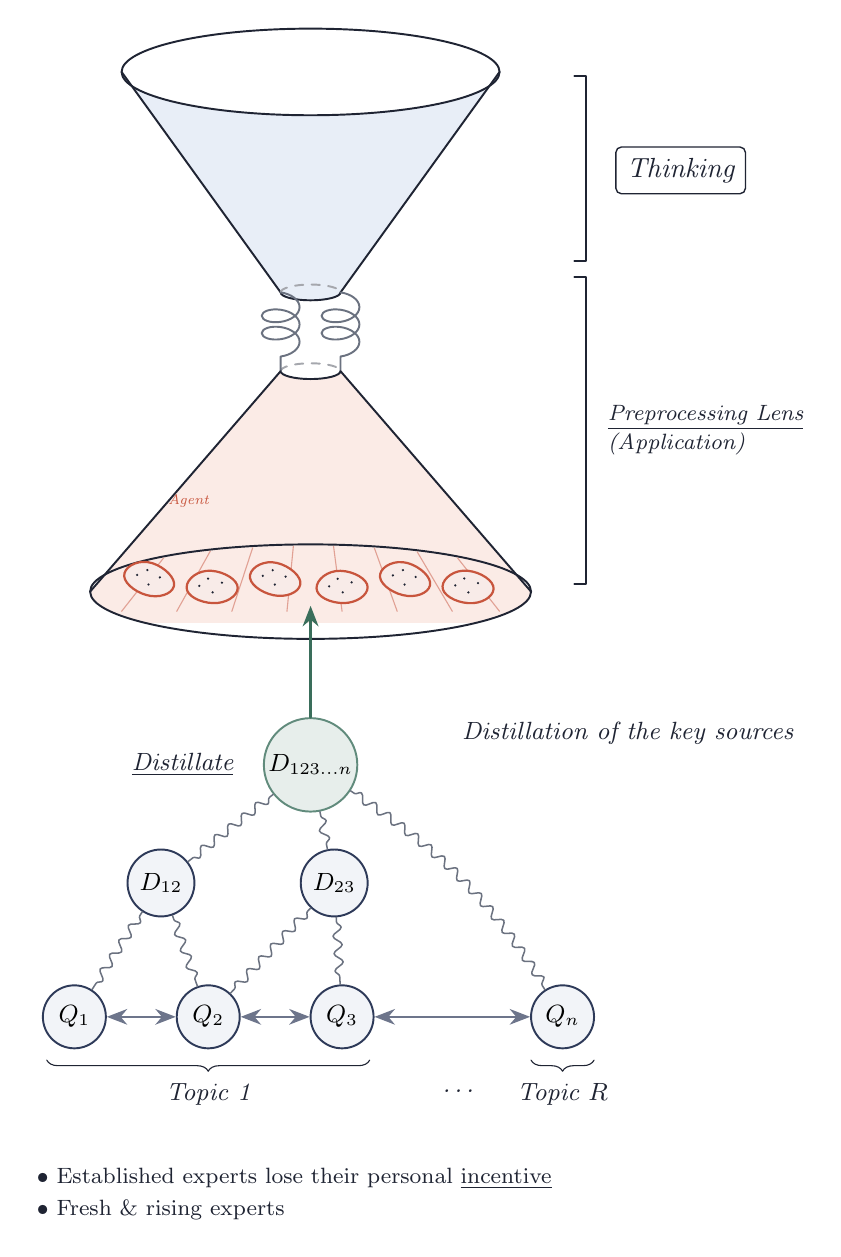
\begin{tikzpicture}[
    line cap=round, line join=round,
    >={Stealth[length=2.6mm, width=2.0mm]},
    %% --- semantic styles ---
    outline/.style   = {draw=ink, line width=0.7pt},
    coilline/.style  = {draw=coil, line width=0.7pt},
    agent/.style     = {draw=lens, line width=0.8pt, fill=lens!12},
    dnode/.style     = {circle, draw=node, line width=0.7pt,
                        fill=nodebg, minimum size=8.5mm,
                        inner sep=1pt, font=\small},
    dlabel/.style    = {font=\itshape\small, text=ink},
    sectionlabel/.style = {font=\itshape, text=ink,
                           draw=ink, line width=0.5pt,
                           rounded corners=2pt,
                           inner sep=4pt, fill=white},
    squiggly/.style  = {draw=soft, line width=0.55pt,
                        decorate, decoration={snake,
                            amplitude=0.55mm, segment length=2.2mm,
                            post length=0.6mm, pre length=0.6mm}},
    flow/.style      = {->, draw=accent, line width=1.1pt},
    sideArrow/.style = {<->, draw=node!70, line width=0.55pt},
    note/.style      = {font=\footnotesize, text=ink, align=left}
]

%% ============================================================
%% HOURGLASS — top funnel (Denken) + coil + bottom funnel (Linse)
%% ============================================================

%% key coordinates
\coordinate (Otop)  at (0, 7.0);   % centre of top opening
\coordinate (Wtop)  at (0, 4.2);   % top of waist
\coordinate (Wbot)  at (0, 3.2);   % bottom of waist
\coordinate (Obot)  at (0, 0.4);   % centre of bottom opening

\def\Rtop{2.4}     % radius of top opening
\def\Ywall{0.55}   % vertical squash for ellipses
\def\Rwaist{0.38}  % radius at the waist
\def\Ywaist{0.10}
\def\Rbot{2.8}     % radius of bottom opening
\def\Ybot{0.60}

%% --- soft fill for the top half (Denken) ---
\begin{scope}
  \clip
    ($(Otop)+(-\Rtop,0)$)
      arc[start angle=180, end angle=360, x radius=\Rtop, y radius=\Ywall]
      -- ($(Wtop)+(\Rwaist,0)$)
      arc[start angle=0,   end angle=-180, x radius=\Rwaist, y radius=\Ywaist]
      -- cycle;
  \fill[thinkbg] (-3,3) rectangle (3,7.6);
\end{scope}

%% --- soft fill for the bottom half (Linse) ---
\begin{scope}
  \clip
    ($(Wbot)+(-\Rwaist,0)$)
      arc[start angle=180, end angle=360, x radius=\Rwaist, y radius=\Ywaist]
      -- ($(Obot)+(\Rbot,0)$)
      arc[start angle=0,   end angle=-180, x radius=\Rbot, y radius=\Ybot]
      -- cycle;
  \fill[lensbg] (-3.2,0) rectangle (3.2,3.4);
\end{scope}

%% --- TOP funnel outline ---
% top opening (ellipse, front + back)
\draw[outline] (Otop) ellipse [x radius=\Rtop, y radius=\Ywall];
% side walls
\draw[outline] ($(Otop)+(-\Rtop,0)$) -- ($(Wtop)+(-\Rwaist,0)$);
\draw[outline] ($(Otop)+( \Rtop,0)$) -- ($(Wtop)+( \Rwaist,0)$);

%% --- Waist coil (the "filter") ---
% top + bottom rims of the coil section
\draw[outline] ($(Wtop)+(-\Rwaist,0)$)
    arc[start angle=180, end angle=360, x radius=\Rwaist, y radius=\Ywaist];
\draw[outline, dashed, draw=ink!40]
    ($(Wtop)+(-\Rwaist,0)$)
    arc[start angle=180, end angle=0, x radius=\Rwaist, y radius=\Ywaist];
\draw[outline] ($(Wbot)+(-\Rwaist,0)$)
    arc[start angle=180, end angle=360, x radius=\Rwaist, y radius=\Ywaist];
\draw[outline, dashed, draw=ink!40]
    ($(Wbot)+(-\Rwaist,0)$)
    arc[start angle=180, end angle=0, x radius=\Rwaist, y radius=\Ywaist];
% the coil itself (two vertical springs on either side)
\draw[coilline,
      decorate, decoration={coil, aspect=0.55,
                            segment length=2.2mm, amplitude=2.4mm}]
    ($(Wtop)+(-\Rwaist,0)$) -- ($(Wbot)+(-\Rwaist,0)$);
\draw[coilline,
      decorate, decoration={coil, aspect=0.55,
                            segment length=2.2mm, amplitude=2.4mm}]
    ($(Wtop)+( \Rwaist,0)$) -- ($(Wbot)+( \Rwaist,0)$);

%% --- BOTTOM funnel outline ---
\draw[outline] ($(Wbot)+(-\Rwaist,0)$) -- ($(Obot)+(-\Rbot,0)$);
\draw[outline] ($(Wbot)+( \Rwaist,0)$) -- ($(Obot)+( \Rbot,0)$);
% bottom ellipse
\draw[outline] (Obot) ellipse [x radius=\Rbot, y radius=\Ybot];

%% --- Agent fan-lines + agent clusters inside the lens ---
\begin{scope}
  % clip to the bottom dish so nothing leaks outside
  \clip (Obot) ellipse [x radius=\Rbot-0.02, y radius=\Ybot-0.02];
  % red light-rays radiating from the waist into the lens
  \foreach \x in {-2.4,-1.7,-1.0,-0.3,0.4,1.1,1.8,2.4} {
    \draw[lens!55, line width=0.4pt] (0,3.2) -- (\x,0.15);
  }
\end{scope}

% Agent clusters (small "amoebas" of data points) along the dish floor
\foreach \cx/\cy/\rot in {
    -2.05/0.55/-8, -1.25/0.45/6, -0.45/0.55/-4,
     0.40/0.45/8,   1.20/0.55/-6,  2.00/0.45/4}
{
  \begin{scope}[shift={(\cx,\cy)}, rotate=\rot]
    \draw[agent] plot[smooth cycle, tension=0.9]
        coordinates {(-0.32,0) (-0.05,0.22) (0.32,0) (0.05,-0.20)};
    \foreach \dx/\dy in {-0.16/0.04, 0/-0.06, 0.13/0.05, -0.04/0.12} {
        \fill[ink] (\dx,\dy) circle (0.45pt);
    }
  \end{scope}
}
% small "Agent" label in red, like the original
\node[font=\tiny\itshape, text=lens] at (-1.55, 1.55) {Agent};

%% ============================================================
%% RIGHT-SIDE BRACKETS + SECTION LABELS
%% ============================================================
\def\BX{3.35} % bracket x-position

% Thinking bracket (top half)
\draw[outline] (\BX,6.95) -- ++(0.15,0) -- ($(\BX+0.15, 4.6)$) -- ++(-0.15,0);
\node[sectionlabel] at (\BX+1.35, 5.75) {Thinking};

% Preprocessing Lens bracket (bottom half)
\draw[outline] (\BX,4.4) -- ++(0.15,0) -- ($(\BX+0.15, 0.5)$) -- ++(-0.15,0);
\node[note, anchor=west] at (\BX+0.30, 2.45)
    {\itshape\underline{Preprocessing Lens}\\[1pt]\itshape (Application)};

%% ============================================================
%% DISTILLATE → SOURCES TREE  (below the hourglass)
%% ============================================================

% Root (Destillat)
\node[dnode, fill=accent!12, draw=accent!80] (Droot)
    at (0, -1.8) {$D_{123\dots n}$};
\node[dlabel, anchor=east] at ($(Droot.west)+(-0.25,0)$)
    {\underline{Distillate}};
\node[dlabel, anchor=west] at (1.8, -1.4)
    {Distillation of the key sources};

% Intermediate distillates
\node[dnode] (D12) at (-1.9, -3.3) {$D_{12}$};
\node[dnode] (D23) at ( 0.3, -3.3) {$D_{23}$};

% Sources Q1..Qn
\node[dnode, minimum size=8mm] (Q1) at (-3.0, -5.0) {$Q_1$};
\node[dnode, minimum size=8mm] (Q2) at (-1.3, -5.0) {$Q_2$};
\node[dnode, minimum size=8mm] (Q3) at ( 0.4, -5.0) {$Q_3$};
\node[dnode, minimum size=8mm] (Qn) at ( 3.2, -5.0) {$Q_n$};

% Distillation links (squiggly = "informal aggregation")
\draw[squiggly] (Droot) -- (D12);
\draw[squiggly] (Droot) -- (D23);
\draw[squiggly] (Droot) to[bend left=12] (Qn);

\draw[squiggly] (D12) -- (Q1);
\draw[squiggly] (D12) -- (Q2);
\draw[squiggly] (D23) -- (Q2);
\draw[squiggly] (D23) -- (Q3);

% Lateral discussion arrows between sources
\draw[sideArrow] (Q1) -- (Q2);
\draw[sideArrow] (Q2) -- (Q3);
\draw[sideArrow] (Q3) -- (Qn);

% Themes (Themen) under the sources
\draw[decorate, decoration={brace, mirror, amplitude=4pt}, draw=ink]
    (-3.35,-5.55) -- (0.75,-5.55)
    node[midway, below=5pt, dlabel] {Topic 1};
\node[dlabel] at (1.9,-5.95) {\ldots};
\draw[decorate, decoration={brace, mirror, amplitude=4pt}, draw=ink]
    (2.8,-5.55) -- (3.6,-5.55)
    node[midway, below=5pt, dlabel] {Topic $R$};

%% --- Flow arrow: distillate → bottom of the lens ---
\draw[flow] (Droot.north) -- ($(Obot)+(0,-0.18)$);

%% ============================================================
%% NOTES UNDER THE DIAGRAM
%% ============================================================
\node[note, anchor=north west] at (-3.6, -6.8)
    {$\bullet$~Established experts lose their
       personal \underline{incentive}\\[2pt]
     $\bullet$~Fresh \& rising experts};

\end{tikzpicture}
}
\end{center}

\newpage

%% ============================================================
%% Stage 2 — Distillation (zoom into one source)
%% ============================================================
\stage{2}{Distillation}{one source $\longrightarrow$ structured distillate $\longrightarrow$ knowledge graph}

Zooming into a single source. Each item is processed through six parallel
\emph{distillation lenses} — Topic, Author, Implicit Assumptions, Theories,
Conclusions, and Methodology. The lens outputs are synthesised into a
multi-dimensional distillate $D_i$, which is then \textbf{pushed into the
knowledge graph} for downstream use.

\vspace{10pt}
\begin{center}
\adjustbox{max width=\textwidth, max height=21cm, center}{%
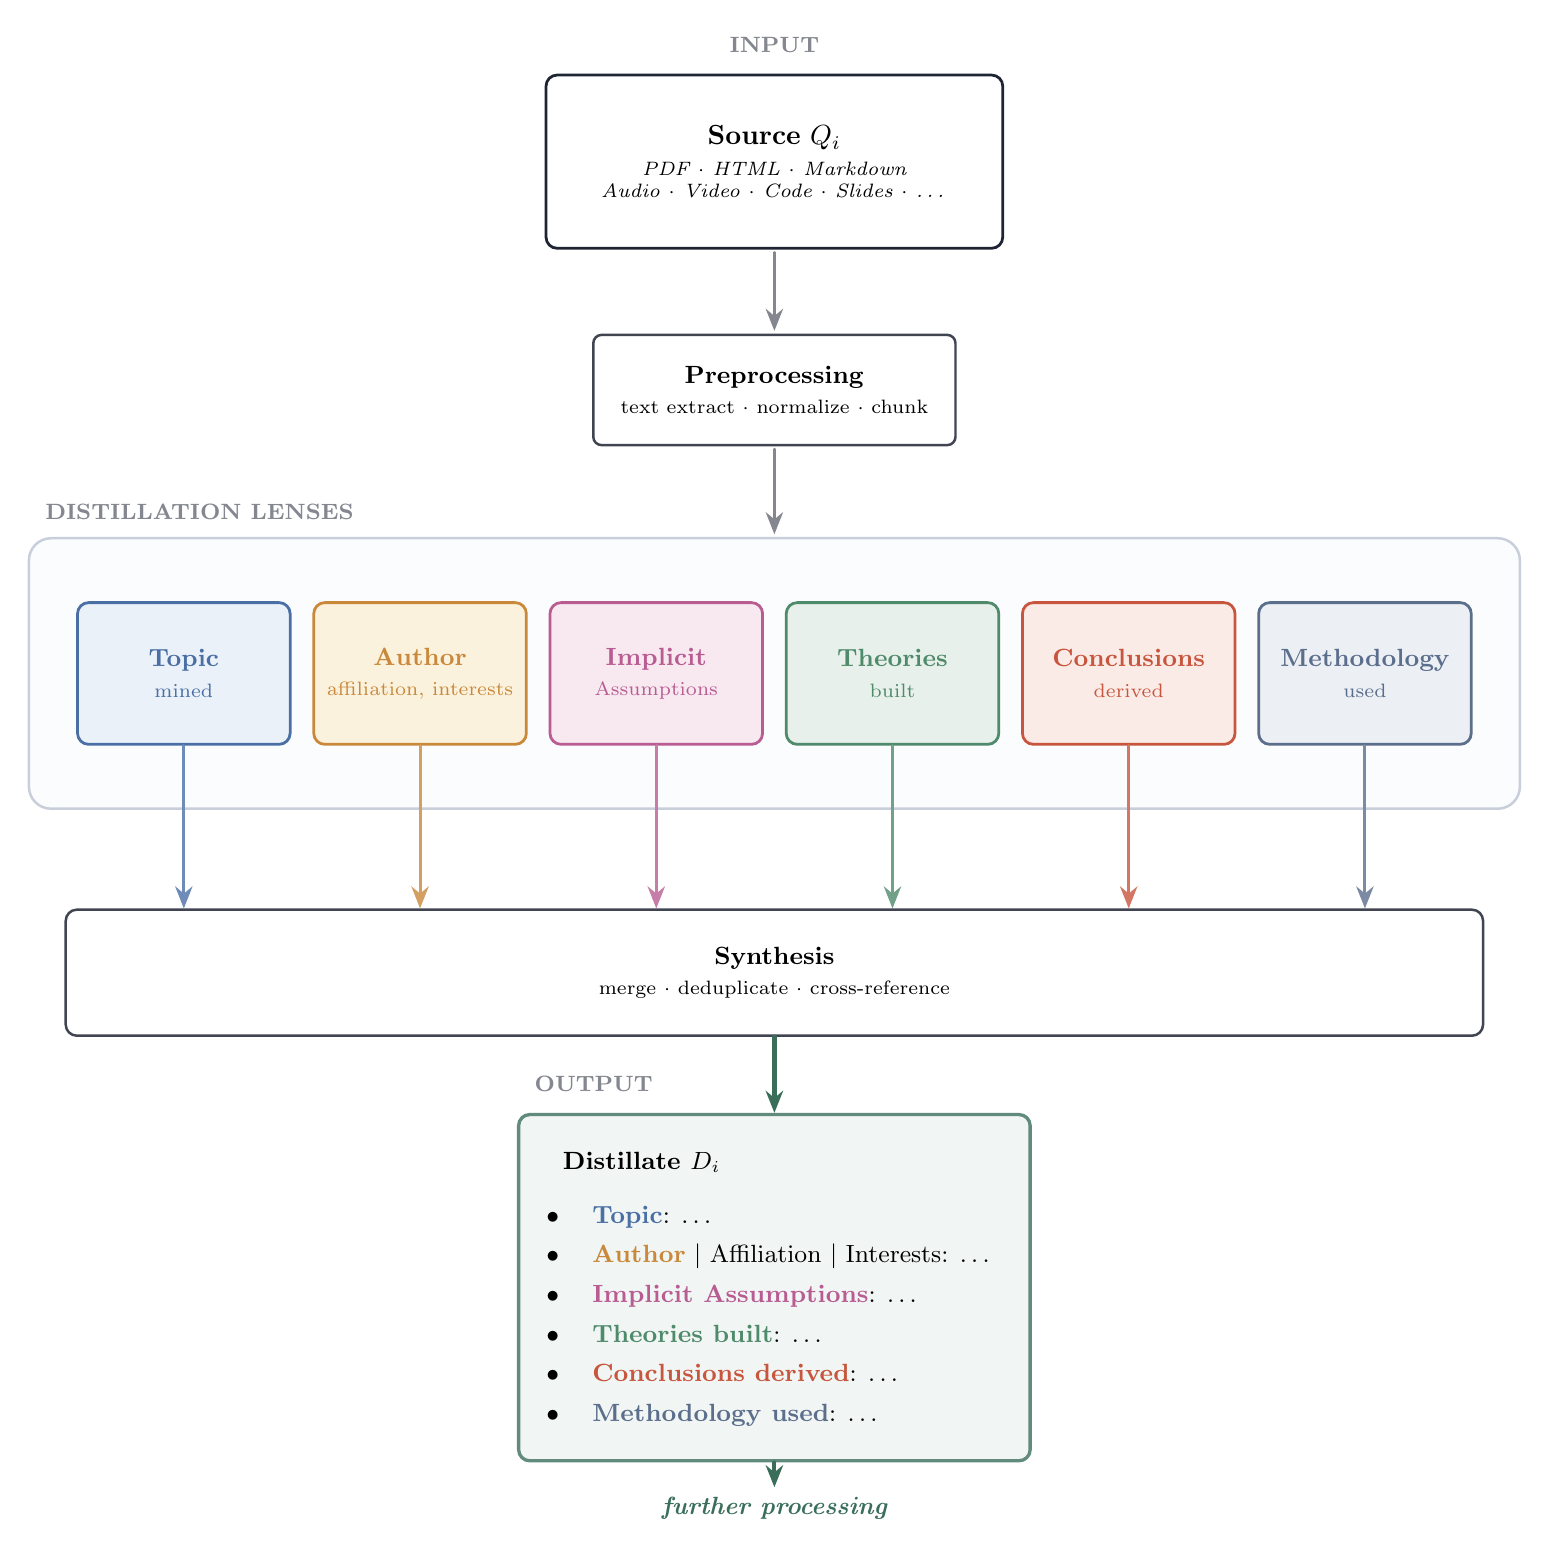
\begin{tikzpicture}[
    line cap=round, line join=round,
    >={Stealth[length=2.8mm, width=2.2mm]},
    %% --- semantic styles ---
    outline/.style       = {draw=ink, line width=0.8pt},
    sourcebox/.style     = {rectangle, draw=ink, fill=white, line width=1pt,
                            rounded corners=4pt, minimum width=58mm,
                            minimum height=22mm, font=\normalsize,
                            align=center},
    procbox/.style       = {rectangle, draw=ink!85, fill=white, line width=0.9pt,
                            rounded corners=3pt, minimum width=46mm,
                            minimum height=14mm, font=\small,
                            align=center, inner sep=4pt},
    synbar/.style        = {rectangle, draw=ink!85, fill=white, line width=0.9pt,
                            rounded corners=4pt, minimum width=180mm,
                            minimum height=16mm, font=\small,
                            align=center, inner sep=4pt},
    lensbox/.style       = {rectangle, line width=1pt, rounded corners=4pt,
                            minimum width=27mm, minimum height=18mm,
                            font=\small\bfseries, align=center, inner sep=3pt},
    distbox/.style       = {rectangle, draw=accent!80, fill=accent!7,
                            line width=1.2pt, rounded corners=4pt,
                            inner sep=10pt, font=\small, align=left},
    keyflow/.style       = {->, draw=accent, line width=1.8pt},
    procflow/.style      = {->, draw=ink!55, line width=1pt,
                            shorten >=1pt, shorten <=1pt},
    sectionlabel/.style  = {font=\footnotesize\bfseries, text=ink!55}
]

%% =====================================================
%% INPUT — Source with format examples
%% =====================================================
\node[sourcebox] (SRC) at (0, 6.5) {%
    \textbf{Source} $Q_i$\\[3pt]
    \begin{minipage}{50mm}\centering
        \scriptsize\itshape
        PDF $\cdot$ HTML $\cdot$ Markdown\\
        Audio $\cdot$ Video $\cdot$ Code $\cdot$ Slides $\cdot$ \ldots
    \end{minipage}
};
\node[sectionlabel, anchor=south] at ($(SRC.north) + (0, 1.5mm)$) {INPUT};

%% =====================================================
%% Preprocessing
%% =====================================================
\node[procbox] (PRE) at (0, 3.6) {%
    \textbf{Preprocessing}\\
    \scriptsize text extract $\cdot$ normalize $\cdot$ chunk
};
\draw[procflow] (SRC) -- (PRE);

%% =====================================================
%% DISTILLATION LENSES — 6 dimensions in a SINGLE ROW
%% =====================================================
\node[lensbox, fill=c1bg, draw=c1, text=c1] (L1) at (-7.5, 0)
    {Topic\\\scriptsize\normalfont mined};
\node[lensbox, fill=c2bg, draw=c2, text=c2] (L2) at (-4.5, 0)
    {Author\\\scriptsize\normalfont affiliation, interests};
\node[lensbox, fill=c3bg, draw=c3, text=c3] (L3) at (-1.5, 0)
    {Implicit\\\scriptsize\normalfont Assumptions};
\node[lensbox, fill=c4bg, draw=c4, text=c4] (L4) at ( 1.5, 0)
    {Theories\\\scriptsize\normalfont built};
\node[lensbox, fill=c5bg, draw=c5, text=c5] (L5) at ( 4.5, 0)
    {Conclusions\\\scriptsize\normalfont derived};
\node[lensbox, fill=c6bg, draw=c6, text=c6] (L6) at ( 7.5, 0)
    {Methodology\\\scriptsize\normalfont used};

% Container around lenses
\begin{scope}[on background layer]
    \node[draw=stageborder, fill=stagebg, rounded corners=8pt,
          line width=0.9pt,
          inner xsep=6mm, inner ysep=8mm,
          fit=(L1) (L6)] (LBOX) {};
\end{scope}
\node[sectionlabel, anchor=south west]
    at ($(LBOX.north west) + (1mm, 1mm)$) {DISTILLATION LENSES};

% Single fan-out from PRE into the lens container
\draw[procflow] (PRE.south) -- (LBOX.north);

%% =====================================================
%% SYNTHESIS — wide bar so every lens drops STRAIGHT down
%% =====================================================
\node[synbar] (SYN) at (0, -3.8) {%
    \textbf{Synthesis}\\
    \scriptsize merge $\cdot$ deduplicate $\cdot$ cross-reference
};

% Six straight vertical colour-coded arrows — no overlap, no curves
\foreach \L/\C in {L1/c1, L2/c2, L3/c3, L4/c4, L5/c5, L6/c6}
    \draw[->, draw=\C!80, line width=1.1pt]
        (\L.south) -- (\L.south |- SYN.north);

%% =====================================================
%% OUTPUT — Distillate as a structured record
%% =====================================================
\node[distbox] (DIST) at (0, -7.8) {%
    \begin{tabular}{@{}rl@{}}
        \multicolumn{2}{l}{\bfseries Distillate $D_i$}\\[5pt]
        $\bullet$ & {\color{c1}\bfseries Topic}: \ldots\\
        $\bullet$ & {\color{c2}\bfseries Author} $\mid$ Affiliation $\mid$ Interests: \ldots\\
        $\bullet$ & {\color{c3}\bfseries Implicit Assumptions}: \ldots\\
        $\bullet$ & {\color{c4}\bfseries Theories built}: \ldots\\
        $\bullet$ & {\color{c5}\bfseries Conclusions derived}: \ldots\\
        $\bullet$ & {\color{c6}\bfseries Methodology used}: \ldots\\
    \end{tabular}
};

\draw[keyflow] (SYN) -- (DIST);
\node[sectionlabel, anchor=south west]
    at ($(DIST.north west) + (1mm, 1.5mm)$) {OUTPUT};

%% =====================================================
%% Further processing
%% =====================================================
\node[font=\small\bfseries\itshape, text=accent] (FP) at (0, -10.6)
    {further processing};
\draw[keyflow, line width=1.4pt] (DIST.south) -- (FP);

\end{tikzpicture}
}
\end{center}

\newpage

%% ============================================================
%% Stage 3 — Knowledge Graph (Source schema)
%% ============================================================
\stage{3}{Knowledge Graph}{per-source schema — where one distillate lands}

Each distillate populates a typed graph with one central
\texttt{Source/Distillate} node and six entity types: \texttt{Author},
\texttt{Topic}, \texttt{Theory}, \texttt{Conclusion}, \texttt{Assumption},
\texttt{Methodology}. Higher-level entities (\texttt{Affiliation},
\texttt{Theme}) emerge as natural groupings. As distillates accumulate, shared
entities — e.g.\ the same Author or Topic across many sources — become hubs
that surface non-trivial cross-source connections.

\vspace{10pt}
\begin{center}
\adjustbox{max width=\textwidth, max height=21cm, center}{%
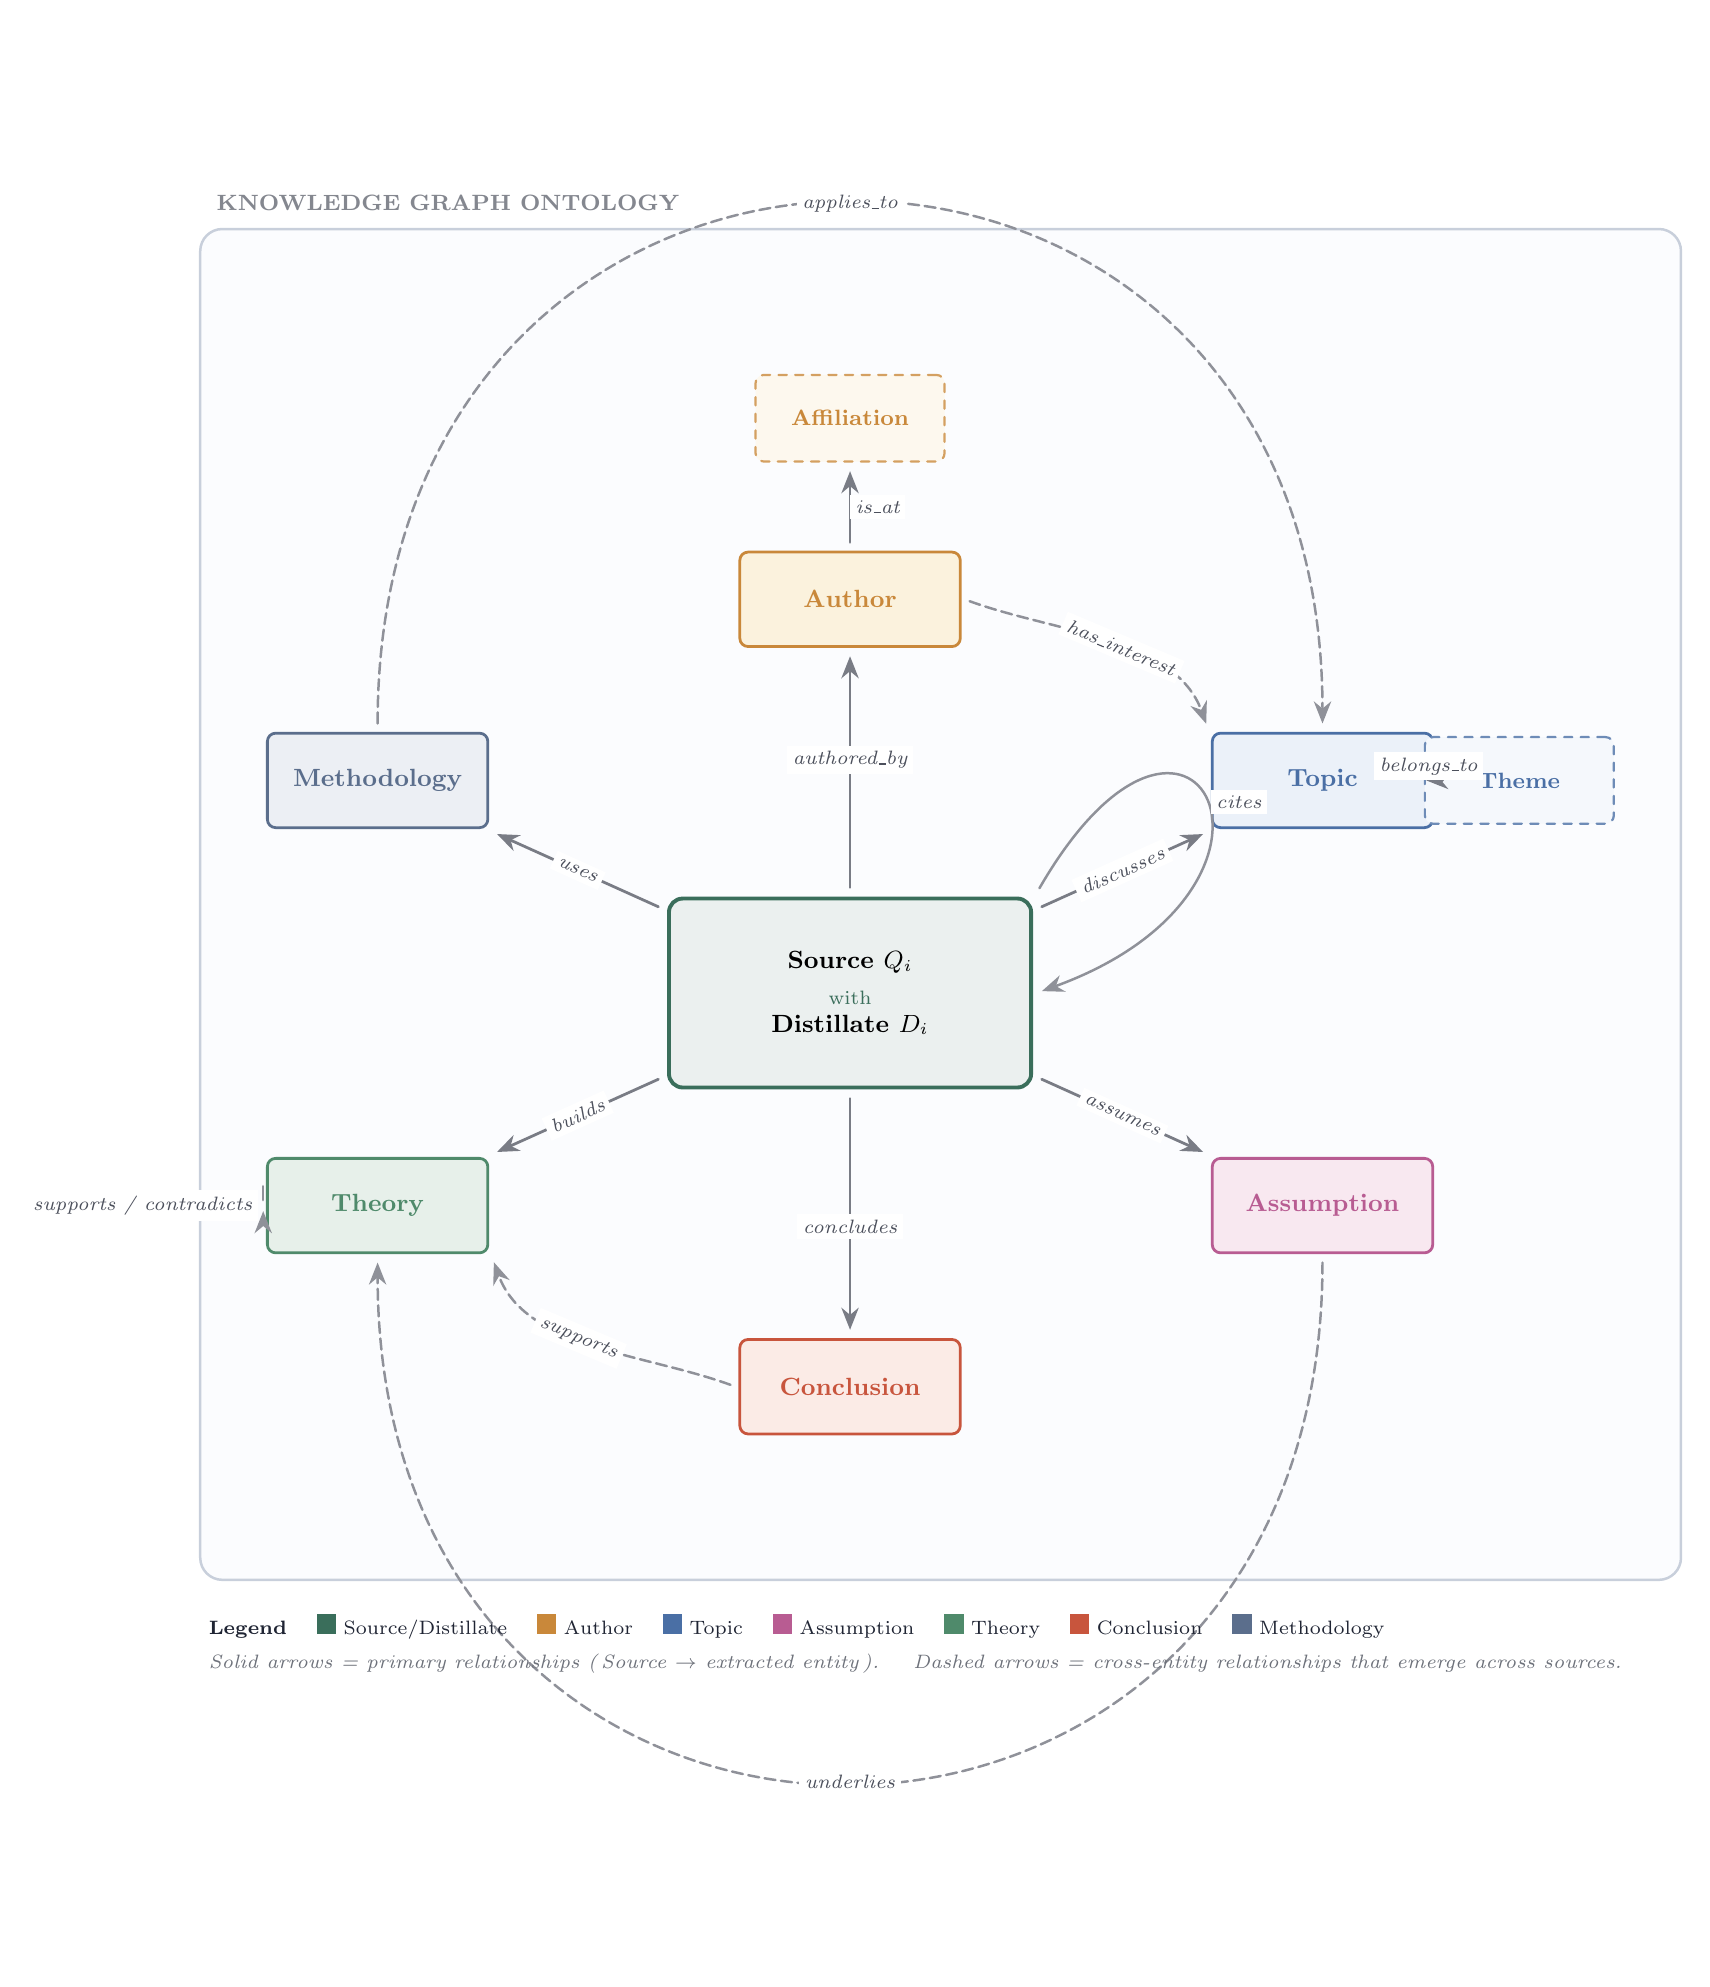
\begin{tikzpicture}[
    line cap=round, line join=round,
    >={Stealth[length=2.8mm, width=2.2mm]},
    %% --- semantic styles ---
    entity/.style       = {rectangle, line width=1pt, rounded corners=3pt,
                           minimum width=28mm, minimum height=12mm,
                           font=\small\bfseries, align=center,
                           inner sep=4pt, outer sep=1.5pt},
    centerentity/.style = {rectangle, draw=accent, fill=accent!10,
                           line width=1.4pt, rounded corners=5pt,
                           minimum width=46mm, minimum height=24mm,
                           font=\small\bfseries, align=center,
                           inner sep=6pt, outer sep=2pt},
    secondary/.style    = {rectangle, line width=0.8pt, rounded corners=3pt,
                           minimum width=24mm, minimum height=11mm,
                           font=\footnotesize\bfseries, align=center,
                           inner sep=3pt, dashed, outer sep=1.5pt},
    primaryedge/.style  = {->, draw=ink!60, line width=1pt,
                           shorten >=2pt, shorten <=2pt},
    crossedge/.style    = {->, draw=ink!50, line width=0.9pt,
                           shorten >=2pt, shorten <=2pt,
                           dash pattern=on 4pt off 2pt},
    selfedge/.style     = {->, draw=ink!50, line width=0.9pt,
                           shorten >=2pt, shorten <=2pt},
    edgelabel/.style    = {font=\scriptsize\itshape, text=ink!80,
                           fill=white, inner sep=2pt, outer sep=0pt},
    sectionlabel/.style = {font=\footnotesize\bfseries, text=ink!55}
]

%% ============================================================
%% CENTER — Source + Distillate
%% ============================================================
\node[centerentity] (S) at (0, 0) {%
    Source $Q_i$\\[2pt]
    {\scriptsize\mdseries\color{accent} with}\\[-1pt]
    Distillate $D_i$
};

%% ============================================================
%% PRIMARY ENTITIES — 6 dimensions, large radial layout
%% ============================================================
\node[entity, fill=c2bg, draw=c2, text=c2] (Author)       at (0,    5.0)  {Author};
\node[entity, fill=c1bg, draw=c1, text=c1] (Topic)        at (6.0,  2.7)  {Topic};
\node[entity, fill=c3bg, draw=c3, text=c3] (Assumption)   at (6.0, -2.7)  {Assumption};
\node[entity, fill=c5bg, draw=c5, text=c5] (Conclusion)   at (0,   -5.0)  {Conclusion};
\node[entity, fill=c4bg, draw=c4, text=c4] (Theory)       at (-6.0,-2.7)  {Theory};
\node[entity, fill=c6bg, draw=c6, text=c6] (Methodology)  at (-6.0, 2.7)  {Methodology};

%% ============================================================
%% SECONDARY ENTITIES — pushed outward, clear of the cross-arcs
%% ============================================================
\node[secondary, fill=c2bg!50, draw=c2!80, text=c2]
    (Affil) at (0,   7.3) {Affiliation};
\node[secondary, fill=c1bg!50, draw=c1!80, text=c1]
    (Theme) at (8.5, 2.7) {Theme};

%% ============================================================
%% PRIMARY EDGES — radial spokes from Source
%% ============================================================
\draw[primaryedge] (S) -- node[edgelabel, pos=0.55]
    {authored\_by} (Author);
\draw[primaryedge] (S) -- node[edgelabel, pos=0.5, sloped]
    {discusses}   (Topic);
\draw[primaryedge] (S) -- node[edgelabel, pos=0.5, sloped]
    {assumes}     (Assumption);
\draw[primaryedge] (S) -- node[edgelabel, pos=0.55]
    {concludes}   (Conclusion);
\draw[primaryedge] (S) -- node[edgelabel, pos=0.5, sloped]
    {builds}      (Theory);
\draw[primaryedge] (S) -- node[edgelabel, pos=0.5, sloped]
    {uses}        (Methodology);

%% ============================================================
%% SECONDARY EDGES — to grouping entities
%% ============================================================
\draw[primaryedge] (Author) -- node[edgelabel, right] {is\_at}      (Affil);
\draw[primaryedge] (Topic)  -- node[edgelabel, above] {belongs\_to} (Theme);

%% ============================================================
%% CROSS-ENTITY EDGES — outer arcs only (no centre crossings)
%% ============================================================
% Author --has_interest--> Topic   (short arc, upper-right outside corner)
\draw[crossedge] (Author.east) to[out=-20, in=110, looseness=0.9]
    node[edgelabel, sloped, pos=0.55] {has\_interest}
    (Topic.north west);

% Methodology --applies_to--> Topic   (long arc OVER the top, above Affiliation)
\draw[crossedge] (Methodology.north) to[out=90, in=90, looseness=1.9]
    node[edgelabel, pos=0.5] {applies\_to}
    (Topic.north);

% Conclusion --supports--> Theory   (short arc, lower-left outside corner)
\draw[crossedge] (Conclusion.west) to[out=160, in=-70, looseness=0.9]
    node[edgelabel, sloped, pos=0.55] {supports}
    (Theory.south east);

% Assumption --underlies--> Theory   (long arc UNDER the bottom)
\draw[crossedge] (Assumption.south) to[out=-90, in=-90, looseness=1.9]
    node[edgelabel, pos=0.5] {underlies}
    (Theory.south);

%% ============================================================
%% SELF-LOOPS
%% ============================================================
% Theory: supports / contradicts  (loop on the left side, well clear)
\draw[selfedge] (Theory.west) to[out=160, in=200, looseness=10]
    node[edgelabel, anchor=east, xshift=-2pt] {supports / contradicts}
    (Theory.west);

% Source: cites  (compact loop inside the centre, north-east corner)
\draw[selfedge] (S.north east) to[out=60, in=20, looseness=8]
    node[edgelabel, anchor=west, xshift=2pt] {cites}
    (S.east);

%% ============================================================
%% Background container — generous padding for the outer arcs
%% ============================================================
\begin{scope}[on background layer]
    \node[draw=kgborder, fill=kgbg, rounded corners=8pt,
          line width=0.9pt,
          inner xsep=8mm, inner ysep=18mm,
          fit=(Author) (Topic) (Assumption) (Conclusion) (Theory)
              (Methodology) (Affil) (Theme) (S)] (KGBOX) {};
\end{scope}

\node[sectionlabel, anchor=south west]
    at ($(KGBOX.north west) + (1mm, 1mm)$) {KNOWLEDGE GRAPH ONTOLOGY};

%% ============================================================
%% Legend
%% ============================================================
\node[anchor=north west, font=\scriptsize, text=ink]
    at ($(KGBOX.south west) + (0, -3mm)$)
    {\textbf{Legend} \quad
     \textcolor{accent}{\rule{2.5mm}{2.5mm}}~Source/Distillate \quad
     \textcolor{c2}{\rule{2.5mm}{2.5mm}}~Author \quad
     \textcolor{c1}{\rule{2.5mm}{2.5mm}}~Topic \quad
     \textcolor{c3}{\rule{2.5mm}{2.5mm}}~Assumption \quad
     \textcolor{c4}{\rule{2.5mm}{2.5mm}}~Theory \quad
     \textcolor{c5}{\rule{2.5mm}{2.5mm}}~Conclusion \quad
     \textcolor{c6}{\rule{2.5mm}{2.5mm}}~Methodology};

\node[anchor=north west, font=\scriptsize\itshape, text=ink!65]
    at ($(KGBOX.south west) + (0, -8mm)$)
    {Solid arrows = primary relationships (\,Source $\to$ extracted entity\,). \quad
     Dashed arrows = cross-entity relationships that emerge across sources.};

\end{tikzpicture}
}
\end{center}

\newpage

%% ============================================================
%% Stage 4 — Complete ontology (cross-tier)
%% ============================================================
\stage{4}{Complete Ontology}{three tiers — Source $\longrightarrow$ Concentrate $\longrightarrow$ Strategy \& Action}

The full system schema spanning all three tiers. \textbf{Tier 1} is the
per-source extraction (one Source $\to$ one Distillate with six dimensions).
\textbf{Tier 2} is the cross-source aggregation into a Concentrate
($D_{1\ldots n}$), grouped by Theme. \textbf{Tier 3} is the Strategy and
Execution Framework, which the Concentrate informs. The dashed orange arc on
the right is the key cross-tier link: \emph{every phase in the Execution
Framework attaches many Distillates back from Tier~1} (many-to-many).

\vspace{10pt}
\begin{center}
\adjustbox{max width=\textwidth, max height=21cm, center}{%
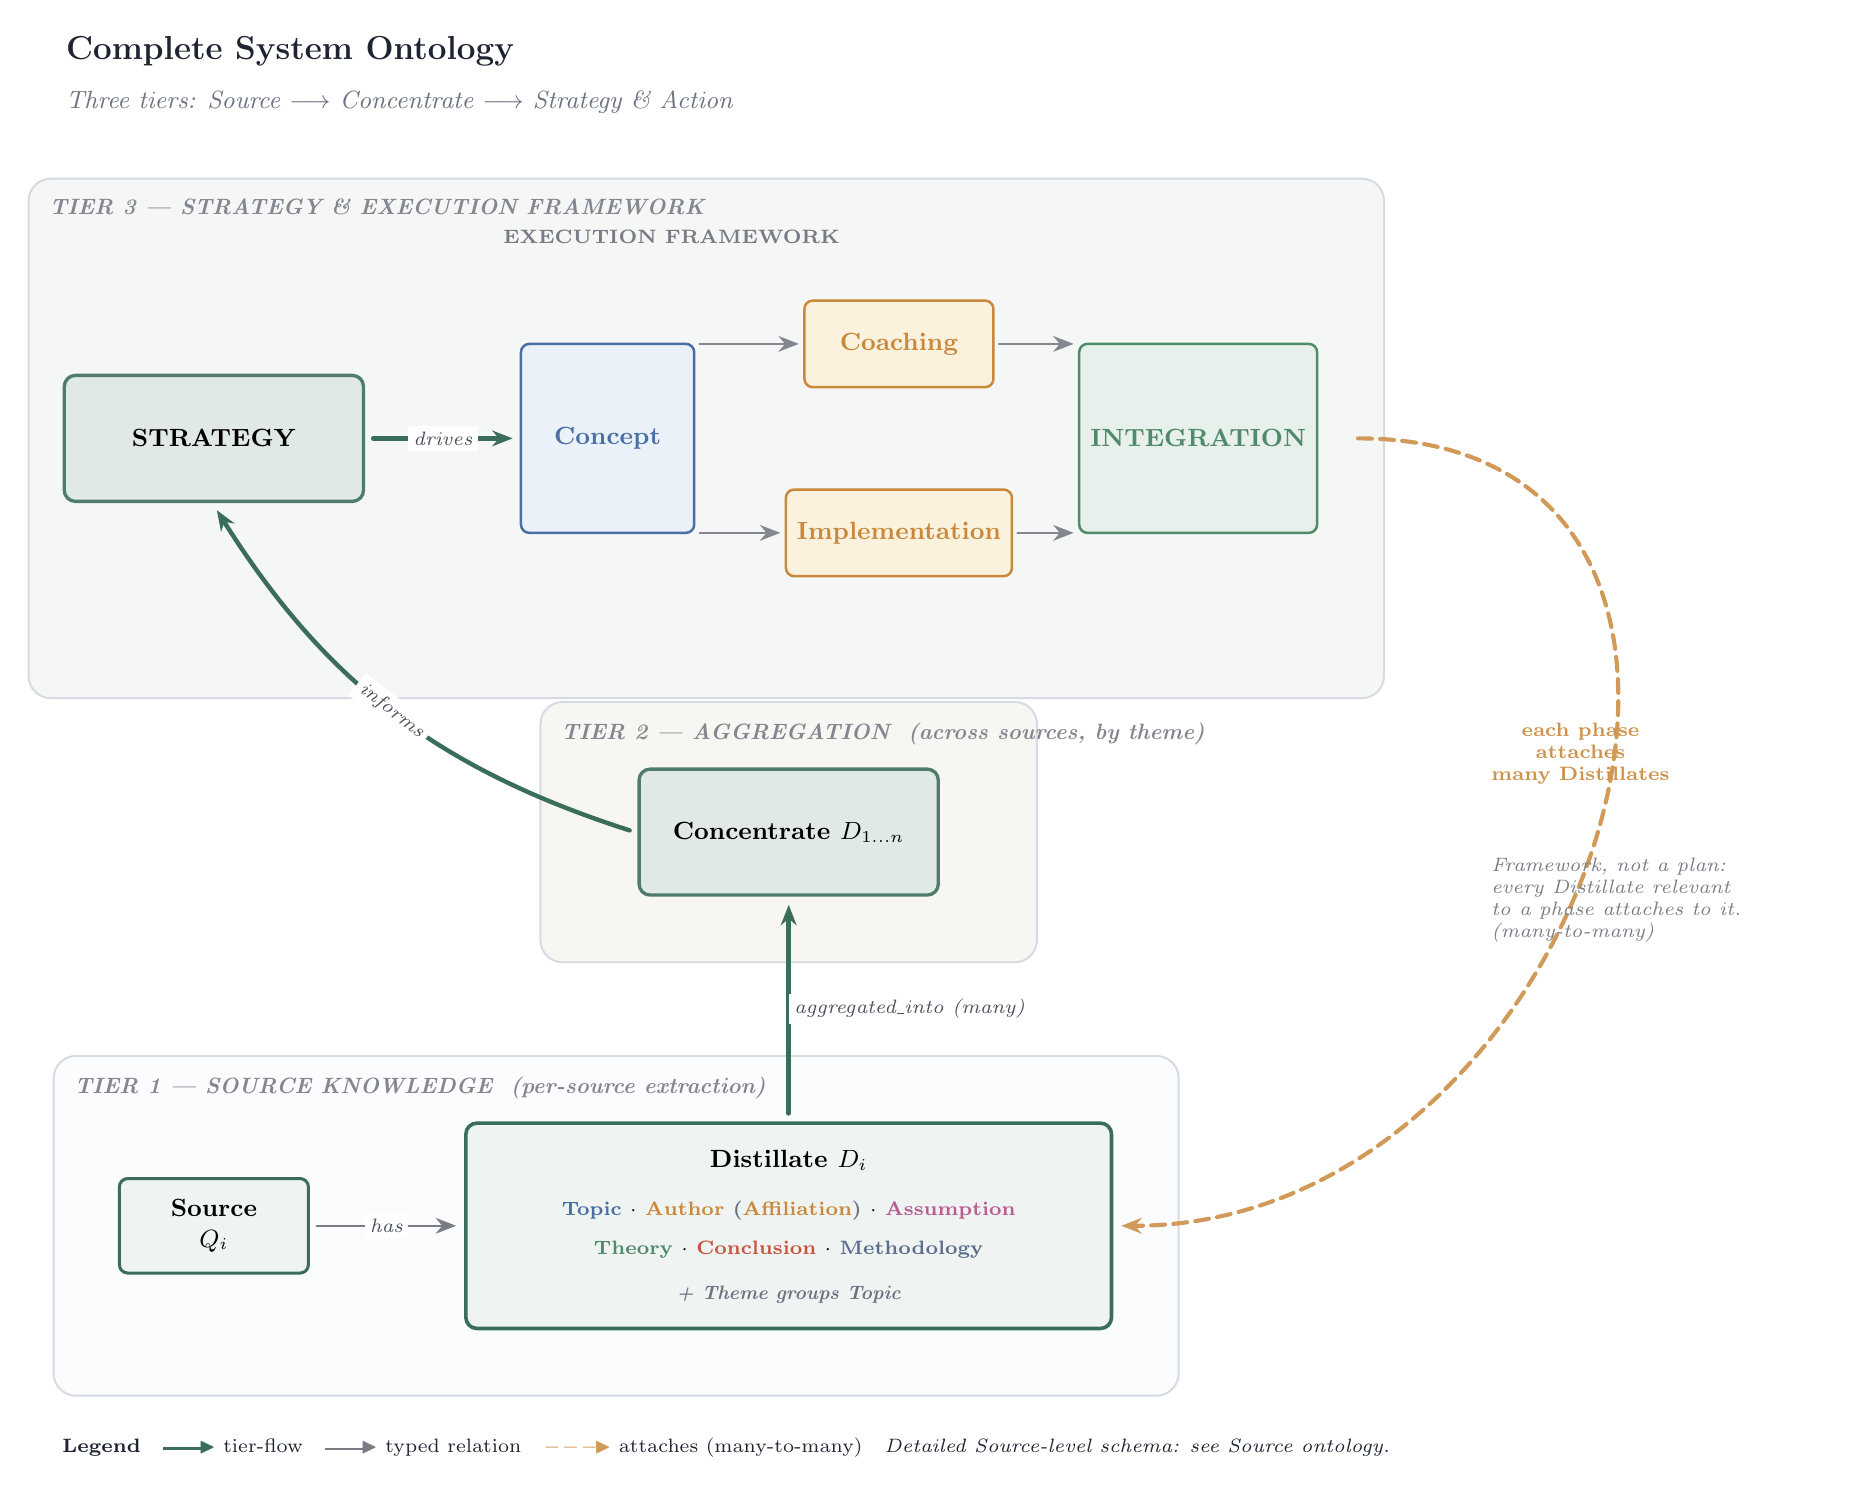
\begin{tikzpicture}[
    line cap=round, line join=round,
    >={Stealth[length=2.6mm, width=2.0mm]},
    entity/.style       = {rectangle, line width=0.9pt, rounded corners=3pt,
                           minimum width=24mm, minimum height=12mm,
                           font=\small\bfseries, align=center,
                           inner sep=4pt, outer sep=1pt},
    distentity/.style   = {rectangle, draw=accent, fill=accent!8,
                           line width=1.3pt, rounded corners=4pt,
                           align=center, inner sep=6pt, outer sep=1.5pt,
                           font=\small\bfseries},
    bigentity/.style    = {rectangle, line width=1.2pt, rounded corners=4pt,
                           minimum width=38mm, minimum height=16mm,
                           font=\small\bfseries, align=center,
                           inner sep=5pt, outer sep=1.5pt},
    pedge/.style        = {->, draw=ink!60, line width=0.9pt,
                           shorten >=2pt, shorten <=2pt},
    tieredge/.style     = {->, draw=accent, line width=1.6pt,
                           shorten >=2pt, shorten <=2pt},
    procflow/.style     = {->, draw=ink!55, line width=0.9pt,
                           shorten >=1pt, shorten <=1pt},
    attachedge/.style   = {->, draw=ph2!85, line width=1.5pt,
                           dash pattern=on 5pt off 3pt,
                           shorten >=2pt, shorten <=2pt},
    edgelabel/.style    = {font=\scriptsize\itshape, text=ink!80,
                           fill=white, inner sep=2pt, outer sep=0pt},
    tierlabel/.style    = {font=\footnotesize\bfseries\itshape, text=ink!55,
                           inner sep=2pt}
]

%% ============================================================
%% Title
%% ============================================================
\node[font=\large\bfseries, text=ink, anchor=south west]
    at (-7.5, 14.6) {Complete System Ontology};
\node[font=\small\itshape, text=soft, anchor=south west]
    at (-7.5, 14.0)
    {Three tiers: Source $\longrightarrow$ Concentrate $\longrightarrow$ Strategy \& Action};

%% ============================================================
%% TIER 1 — Source-level (compact; details in dedicated diagram)
%% ============================================================
\node[entity, fill=accent!8, draw=accent, line width=1.1pt]
    (Source) at (-5.5, 0) {Source\\$Q_i$};

\node[distentity, minimum width=82mm] (Dist) at (1.8, 0) {%
    \begin{tabular}{@{}c@{}}
        \bfseries Distillate $D_i$\\[3pt]
        {\scriptsize
            \textcolor{c1}{\bfseries Topic} $\cdot$
            \textcolor{c2}{\bfseries Author}
            {\color{soft}(\textcolor{c2}{Affiliation})} $\cdot$
            \textcolor{c3}{\bfseries Assumption}}\\
        {\scriptsize
            \textcolor{c4}{\bfseries Theory} $\cdot$
            \textcolor{c5}{\bfseries Conclusion} $\cdot$
            \textcolor{c6}{\bfseries Methodology}}\\[2pt]
        {\scriptsize\color{soft}\itshape + Theme groups Topic}
    \end{tabular}%
};

\draw[pedge] (Source) -- node[edgelabel] {has} (Dist);

% Tier 1 background
\begin{scope}[on background layer]
    \node[draw=tborder, fill=t1bg, rounded corners=8pt, line width=0.7pt,
          inner xsep=8mm, inner ysep=8mm,
          fit=(Source) (Dist)] (T1) {};
\end{scope}
\node[tierlabel, anchor=north west] at ($(T1.north west) + (2mm, -2mm)$)
    {TIER 1\ \textemdash\ SOURCE KNOWLEDGE \ (per-source extraction)};

%% ============================================================
%% TIER 2 — Aggregation
%% ============================================================
\node[bigentity, fill=accent!15, draw=accent!90]
    (Concentrate) at (1.8, 5.0) {Concentrate $D_{1\ldots n}$};

% Tier 2 background
\begin{scope}[on background layer]
    \node[draw=tborder, fill=t2bg, rounded corners=8pt, line width=0.7pt,
          inner xsep=12mm, inner ysep=8mm,
          fit=(Concentrate)] (T2) {};
\end{scope}
\node[tierlabel, anchor=north west] at ($(T2.north west) + (2mm, -2mm)$)
    {TIER 2\ \textemdash\ AGGREGATION \ (across sources, by theme)};

% Edge: Distillate aggregated into Concentrate
\draw[tieredge] (Dist.north) -- node[edgelabel, right]
    {aggregated\_into (many)} (Concentrate.south);

%% ============================================================
%% TIER 3 — Strategy + Execution Framework
%% ============================================================
\node[bigentity, fill=accent!15, draw=accent!90] (Strategy) at (-5.5, 10.0) {STRATEGY};

\node[entity, fill=ph1bg, draw=ph1, text=ph1,
      minimum width=22mm, minimum height=24mm]
    (Concept) at (-0.5, 10.0) {Concept};
\node[entity, fill=ph2bg, draw=ph2, text=ph2,
      minimum width=24mm, minimum height=11mm]
    (Coaching) at (3.2, 11.2) {Coaching};
\node[entity, fill=ph2bg, draw=ph2, text=ph2,
      minimum width=24mm, minimum height=11mm]
    (Impl) at (3.2,  8.8) {Implementation};
\node[entity, fill=ph3bg, draw=ph3, text=ph3,
      minimum width=22mm, minimum height=24mm]
    (Integ) at (7.0, 10.0) {INTEGRATION};

\draw[procflow] (Concept.east |- Coaching.west) -- (Coaching.west);
\draw[procflow] (Concept.east |- Impl.west)     -- (Impl.west);
\draw[procflow] (Coaching.east) -- (Integ.west |- Coaching.east);
\draw[procflow] (Impl.east)     -- (Integ.west |- Impl.east);

% Framework container
\begin{scope}[on background layer]
    \node[draw=ink!25, fill=white, rounded corners=5pt, line width=0.8pt,
          inner xsep=4mm, inner ysep=5mm,
          fit=(Concept) (Coaching) (Impl) (Integ)] (Framework) {};
\end{scope}
\node[font=\scriptsize\bfseries, text=ink!60, anchor=south west]
    at ($(Framework.north west) + (1mm, 0.5mm)$) {EXECUTION FRAMEWORK};

% Strategy/Concentrate connections
\draw[tieredge] (Concentrate.west) to[bend left=20]
    node[edgelabel, sloped, pos=0.5] {informs} (Strategy.south);
\draw[tieredge] (Strategy.east) -- node[edgelabel] {drives} (Concept.west);

% Tier 3 background
\begin{scope}[on background layer]
    \node[draw=tborder, fill=t3bg, rounded corners=8pt, line width=0.7pt,
          inner xsep=4mm, inner ysep=10mm,
          fit=(Strategy) (Framework)] (T3) {};
\end{scope}
\node[tierlabel, anchor=north west] at ($(T3.north west) + (2mm, -2mm)$)
    {TIER 3\ \textemdash\ STRATEGY \& EXECUTION FRAMEWORK};

%% ============================================================
%% Cross-tier ATTACHES (the key new insight)
%% ============================================================
% Wide arc on the right: Framework → Distillate (many-to-many attachment)
\draw[attachedge]
    (Framework.east) to[out=0, in=0, looseness=1.5]
    (Dist.east);

\node[font=\scriptsize\bfseries, text=ph2!90, align=center, anchor=west]
    at (10.6, 6.0)
    {each phase\\\textbf{attaches}\\many Distillates};

\node[font=\scriptsize\itshape, text=ink!60, align=left, anchor=north west]
    at (10.6, 4.8)
    {\textit{Framework, not a plan:}\\
     every Distillate relevant\\
     to a phase attaches to it.\\
     (many-to-many)};

%% ============================================================
%% Legend
%% ============================================================
\node[anchor=north west, font=\scriptsize, text=ink]
    at ($(T1.south west) + (0, -4mm)$)
    {\textbf{Legend}\quad
     \textcolor{accent}{\rule[0.3ex]{5mm}{1pt}\!$\blacktriangleright$}~tier-flow\quad
     \textcolor{ink!60}{\rule[0.3ex]{5mm}{0.6pt}\!$\blacktriangleright$}~typed relation\quad
     \textcolor{ph2!85}{$-\!-\!-$\!$\blacktriangleright$}~attaches (many-to-many)\quad
     \emph{Detailed Source-level schema: see Source ontology.}};

\end{tikzpicture}
}
\end{center}

\newpage

%% ============================================================
%% Stage 5 — Execution Framework
%% ============================================================
\stage{5}{Execution Framework}{not a plan — a framework that distillates \textbf{attach} to}

Execution is \emph{not} a linear plan from Strategy through the four phases.
It is a \textbf{framework}: each phase — \emph{Concept}, \emph{Coaching},
\emph{Implementation}, \emph{Integration} — is a slot that distilled
information can attach to. Deriving the Concept, for example, rests on a
collection of Topics, each containing many Distillates. The internal
arrows show how phases relate to each other; the deeper relationship —
that every Distillate relevant to a phase is attached to it — is what
makes the framework actionable.

\vspace{10pt}
\begin{center}
\adjustbox{max width=\textwidth, max height=21cm, center}{%
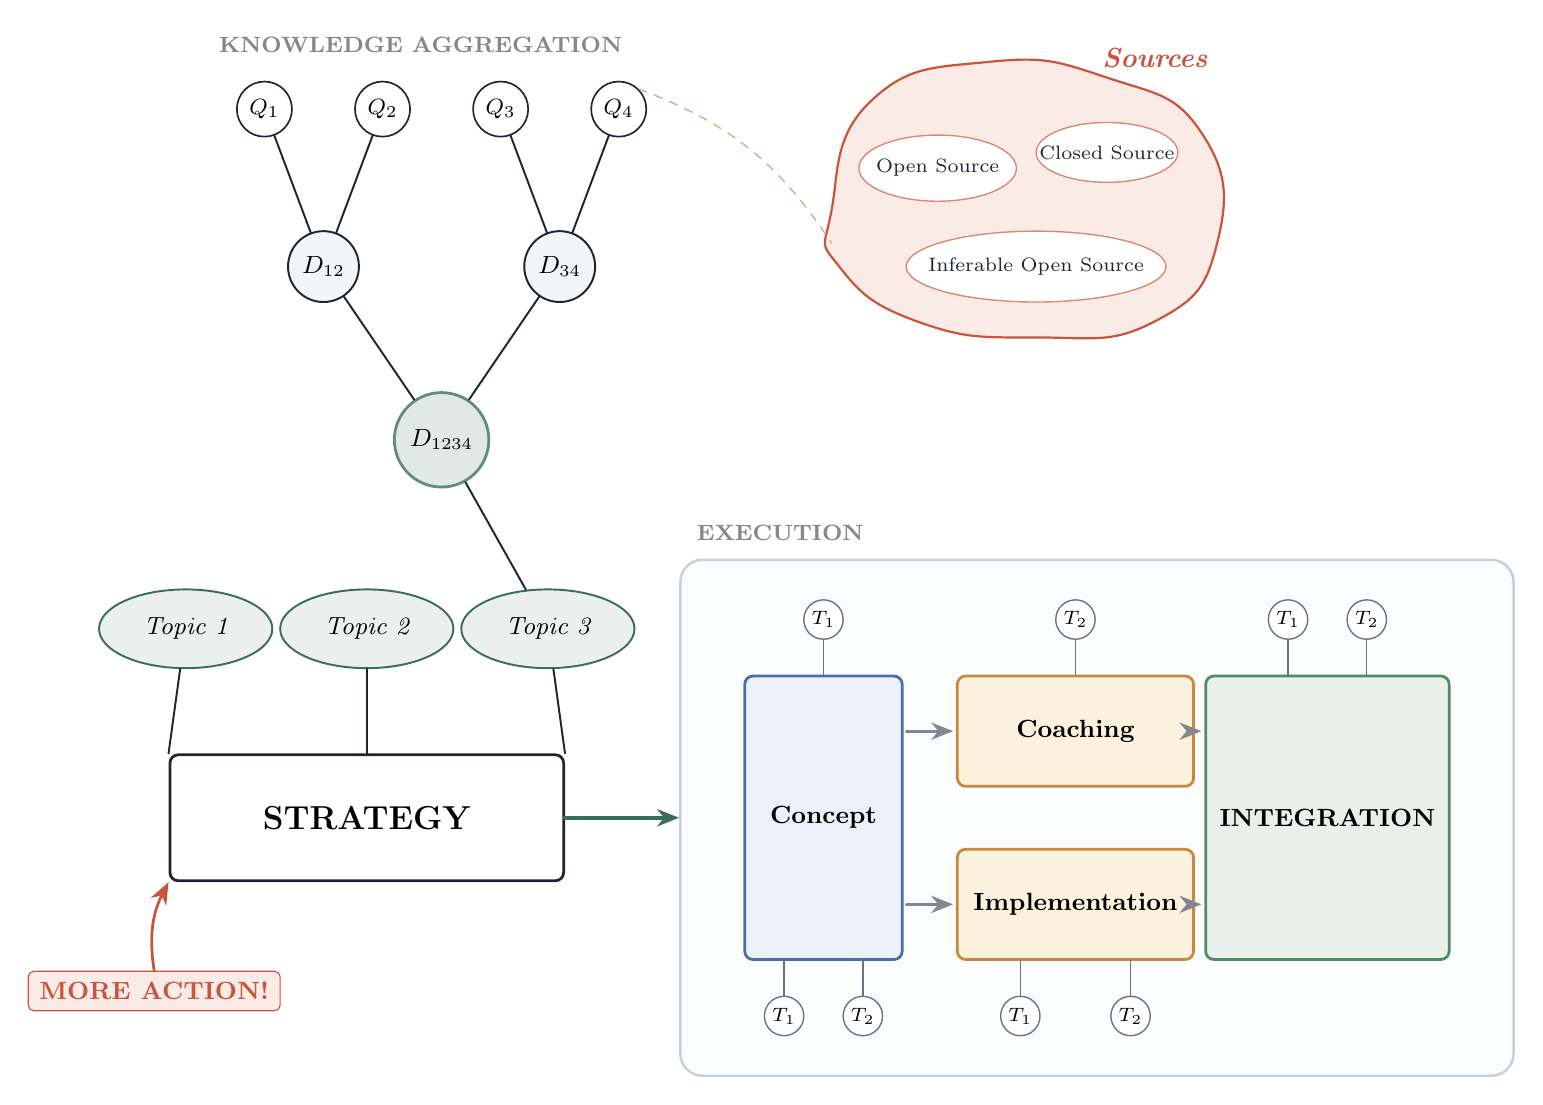
\begin{tikzpicture}[
    line cap=round, line join=round,
    >={Stealth[length=2.8mm, width=2.2mm]},
    %% --- semantic styles ---
    outline/.style      = {draw=ink, line width=0.7pt},
    thinline/.style     = {draw=soft, line width=0.5pt},
    qnode/.style        = {circle, draw=ink, line width=0.6pt, fill=white,
                           minimum size=7mm, inner sep=1pt, font=\footnotesize},
    dnode/.style        = {circle, draw=ink, line width=0.7pt, fill=nodebg,
                           minimum size=9mm, inner sep=1pt, font=\small},
    rootnode/.style     = {circle, draw=accent!80, line width=1pt, fill=accent!15,
                           minimum size=12mm, inner sep=1pt, font=\small},
    topic/.style        = {ellipse, draw=accent, fill=accent!10, line width=0.7pt,
                           minimum width=22mm, minimum height=10mm,
                           font=\small\itshape},
    sbox/.style         = {rectangle, draw=ink, fill=white, line width=1pt,
                           rounded corners=3pt, minimum width=50mm,
                           minimum height=16mm, font=\large\bfseries,
                           align=center},
    pbox/.style         = {rectangle, draw=ink!85, fill=white, line width=0.9pt,
                           rounded corners=3pt, font=\small\bfseries,
                           align=center, inner sep=5pt},
    keyflow/.style      = {->, draw=accent, line width=1.6pt},
    procflow/.style     = {->, draw=ink!55, line width=1pt,
                           shorten >=1pt, shorten <=1pt},
    tinynode/.style     = {circle, draw=soft, line width=0.5pt, fill=white,
                           minimum size=5mm, inner sep=0pt, font=\scriptsize},
    sectionlabel/.style = {font=\footnotesize\bfseries, text=ink!55},
    callout/.style      = {font=\small\bfseries, text=lens, draw=lens,
                           fill=lensbg, rounded corners=2pt, inner sep=4pt}
]

%% ================================================================
%% TOP-LEFT — Knowledge aggregation tree
%% ================================================================
\node[qnode] (Q1) at (-4.0, 8.0) {$Q_1$};
\node[qnode] (Q2) at (-2.5, 8.0) {$Q_2$};
\node[qnode] (Q3) at (-1.0, 8.0) {$Q_3$};
\node[qnode] (Q4) at ( 0.5, 8.0) {$Q_4$};

\node[dnode] (D12)   at (-3.25, 6.0) {$D_{12}$};
\node[dnode] (D34)   at (-0.25, 6.0) {$D_{34}$};
\node[rootnode] (D1234) at (-1.75, 3.8) {$D_{1234}$};

\foreach \a/\b in {Q1/D12, Q2/D12, Q3/D34, Q4/D34, D12/D1234, D34/D1234}
    \draw[outline] (\a) -- (\b);

\node[sectionlabel, anchor=south west] at (-4.7, 8.6)
    {KNOWLEDGE AGGREGATION};

%% ================================================================
%% TOP-RIGHT — Source taxonomy cloud
%% ================================================================
\begin{scope}[shift={(5.6, 6.7)}]
    \draw[lens, fill=lensbg, line width=0.8pt]
        plot[smooth cycle, tension=0.85] coordinates {
            (-2.4,  0.0) (-1.9,  1.4) (-0.4,  1.9) ( 1.1,  1.7)
            ( 2.3,  1.0) ( 2.5, -0.4) ( 1.7, -1.4) ( 0.2, -1.6)
            (-1.3, -1.4) (-2.3, -0.7)
        };
    \node[font=\itshape\bfseries, text=lens, anchor=south east]
        at (2.5, 1.7) {Sources};

    \draw[lens!70, line width=0.5pt, fill=white]
        (-1.05, 0.55) ellipse (1.00 and 0.42);
    \node[font=\scriptsize, text=ink] at (-1.05, 0.55) {Open Source};

    \draw[lens!70, line width=0.5pt, fill=white]
        ( 1.10, 0.75) ellipse (0.90 and 0.38);
    \node[font=\scriptsize, text=ink] at ( 1.10, 0.75) {Closed Source};

    \draw[lens!70, line width=0.5pt, fill=white]
        ( 0.20, -0.70) ellipse (1.65 and 0.45);
    \node[font=\scriptsize, text=ink] at ( 0.20, -0.70) {Inferable Open Source};
\end{scope}

% subtle hint that Q's are drawn from the source pool
\draw[dashed, lens!55, line width=0.5pt]
    (Q4.north east) to[bend left=18]
    ($(5.6, 6.7) + (-2.4, -0.4)$);

%% ================================================================
%% MIDDLE — Topics → STRATEGY
%% ================================================================
\node[topic] (Top1) at (-5.0, 1.4) {Topic 1};
\node[topic] (Top2) at (-2.7, 1.4) {Topic 2};
\node[topic] (Top3) at (-0.4, 1.4) {Topic 3};

\draw[outline] (D1234) -- (Top3);

\node[sbox] (STRAT) at (-2.7, -1.0) {STRATEGY};
\draw[outline] (Top1) -- (STRAT.north west);
\draw[outline] (Top2) -- (STRAT.north);
\draw[outline] (Top3) -- (STRAT.north east);

%% ================================================================
%% RIGHT — EXECUTION container with process flow
%% ================================================================
% Phase 1 — Concept (tall left bar)
\node[pbox, fill=phase1bg, draw=phase1, line width=1pt,
      minimum width=20mm, minimum height=36mm]
    (CONCEPT) at (3.1, -1.0) {Concept};

% Phase 2 — parallel streams (Coaching above, Implementation below)
\node[pbox, fill=phase2bg, draw=phase2, line width=1pt,
      minimum width=30mm, minimum height=14mm]
    (COACH) at (6.3, 0.1) {Coaching};
\node[pbox, fill=phase2bg, draw=phase2, line width=1pt,
      minimum width=30mm, minimum height=14mm]
    (IMPL)  at (6.3, -2.1) {Implementation};

% Phase 3 — Integration (tall right bar)
\node[pbox, fill=phase3bg, draw=phase3, line width=1pt,
      minimum width=22mm, minimum height=36mm,
      font=\small\bfseries]
    (INTEG) at (9.5, -1.0) {INTEGRATION};

% --- Internal process flow arrows ---
\draw[procflow] (CONCEPT.east |- COACH.west) -- (COACH.west);
\draw[procflow] (CONCEPT.east |- IMPL.west)  -- (IMPL.west);
\draw[procflow] (COACH.east)  -- (INTEG.west |- COACH.east);
\draw[procflow] (IMPL.east)   -- (INTEG.west |- IMPL.east);

% --- T markers as inputs (above each phase) ---
\node[tinynode] (Tc_in)  at ($(CONCEPT.north) + (0,    7mm)$) {$T_1$};
\node[tinynode] (Tco_in) at ($(COACH.north)   + (0,    7mm)$) {$T_2$};
\node[tinynode] (Ti1_in) at ($(INTEG.north)   + (-5mm, 7mm)$) {$T_1$};
\node[tinynode] (Ti2_in) at ($(INTEG.north)   + ( 5mm, 7mm)$) {$T_2$};

\draw[thinline] (Tc_in)  -- (CONCEPT.north);
\draw[thinline] (Tco_in) -- (COACH.north);
\draw[thinline] (Ti1_in) -- ($(INTEG.north) + (-5mm, 0)$);
\draw[thinline] (Ti2_in) -- ($(INTEG.north) + ( 5mm, 0)$);

% --- T markers as outputs (below) ---
\node[tinynode] (Tc1_out) at ($(CONCEPT.south) + (-5mm, -7mm)$) {$T_1$};
\node[tinynode] (Tc2_out) at ($(CONCEPT.south) + ( 5mm, -7mm)$) {$T_2$};
\node[tinynode] (Tu1_out) at ($(IMPL.south)    + (-7mm, -7mm)$) {$T_1$};
\node[tinynode] (Tu2_out) at ($(IMPL.south)    + ( 7mm, -7mm)$) {$T_2$};

\draw[thinline] ($(CONCEPT.south) + (-5mm, 0)$) -- (Tc1_out);
\draw[thinline] ($(CONCEPT.south) + ( 5mm, 0)$) -- (Tc2_out);
\draw[thinline] ($(IMPL.south)    + (-7mm, 0)$) -- (Tu1_out);
\draw[thinline] ($(IMPL.south)    + ( 7mm, 0)$) -- (Tu2_out);

% --- Container box (background layer, auto-fitted) ---
\begin{scope}[on background layer]
    \node[draw=execborder, fill=execbg, rounded corners=8pt,
          line width=0.9pt,
          inner xsep=8mm, inner ysep=5mm,
          fit=(CONCEPT) (COACH) (IMPL) (INTEG)
              (Tc_in) (Tco_in) (Ti1_in) (Ti2_in)
              (Tc1_out) (Tc2_out) (Tu1_out) (Tu2_out)]
          (EXECBOX) {};
\end{scope}

% Container title
\node[sectionlabel, anchor=south west]
    at ($(EXECBOX.north west) + (1mm, 1mm)$) {EXECUTION};

% --- Key arrow: STRATEGY → EXECUTION ---
\draw[keyflow] (STRAT.east) -- (EXECBOX.west |- STRAT.east);

%% ================================================================
%% "MORE ACTION!" sticky-note callout
%% ================================================================
\node[callout] (MA) at (-5.4, -3.2) {MORE ACTION!};
\draw[->, lens, line width=1pt]
    (MA.north) to[bend left=18] (STRAT.south west);

\end{tikzpicture}
}
\end{center}

\end{document}